\section{Efficiency and rejection plots for tracker isolation}
\label{app:plots_tk}
In this appendix efficiency and background rejection plots are shown. 
The cut values to determine the curves are superimposed to the plots.

\begin{figure}[htbp]
\begin{center}
 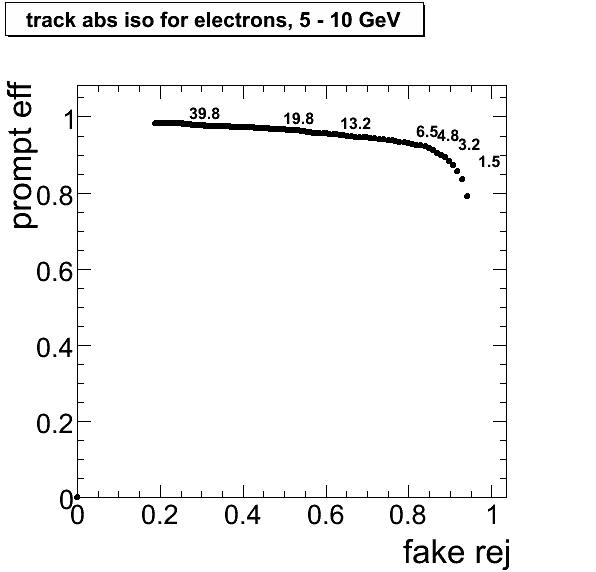
\includegraphics[width = 0.4\textwidth]{pictures/bkgdRej_sigEff/onlyTrack_elec_fake_ptCut0_ptCut1.png}
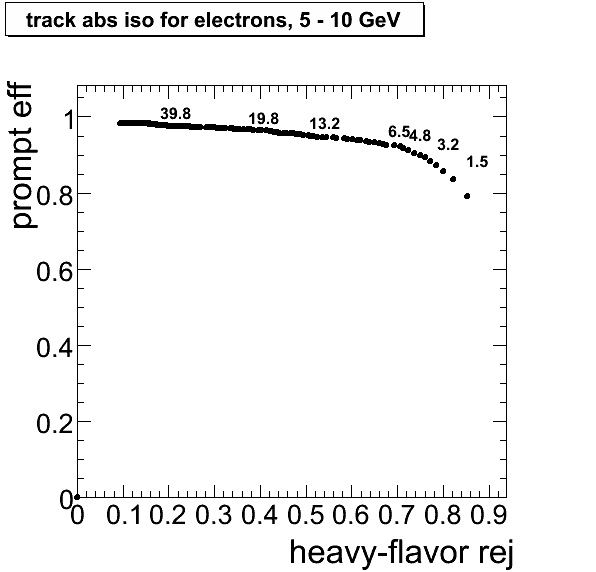
\includegraphics[width = 0.4\textwidth]{pictures/bkgdRej_sigEff/onlyTrack_elec_nonPrompt_ptCut0_ptCut1.png}
\caption{\small{Prompt leptons efficiency with respect to background 
rejection for fake (left) and HF leptons (right) in pT region
from 5 to 10 GeV for electrons. 
Cut values are superimposed to the curve.}\label{fig:rej_el1}}
\end{center}
\end{figure}
\begin{figure}[htbp]
\begin{center}
 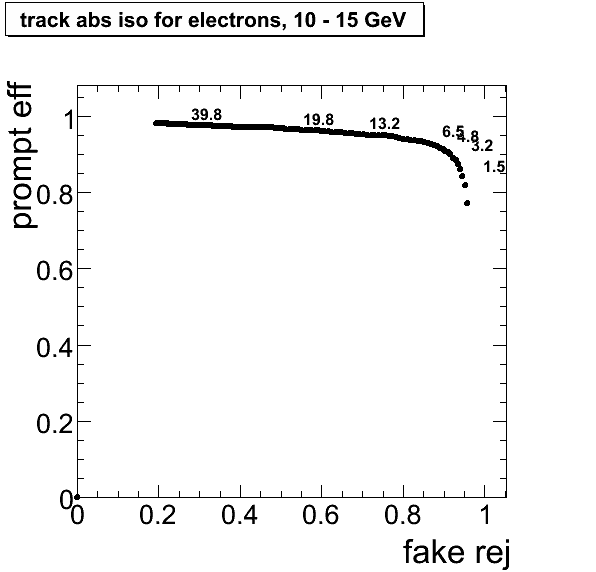
\includegraphics[width = 0.4\textwidth]{pictures/bkgdRej_sigEff/onlyTrack_elec_fake_ptCut1_ptCut2.png}
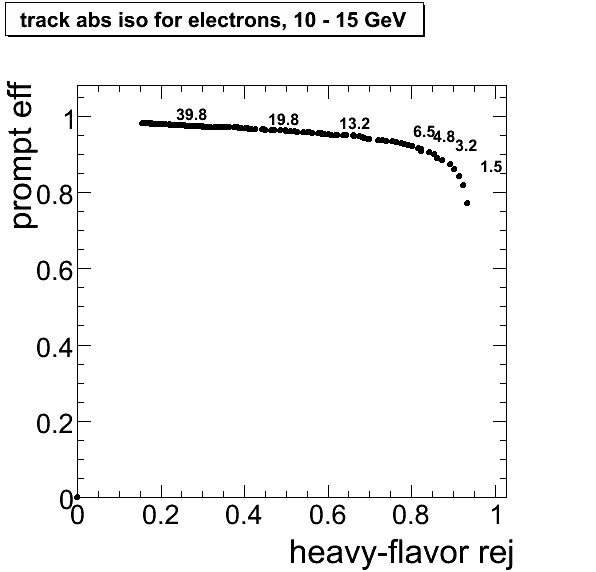
\includegraphics[width = 0.4\textwidth]{pictures/bkgdRej_sigEff/onlyTrack_elec_nonPrompt_ptCut1_ptCut2.png}
\caption{\small{Prompt leptons efficiency with respect to background 
rejection for fake (left) and HF leptons (right) in pT region
from 10 to 15 GeV for electrons. 
Cut values are superimposed to the curve.}\label{fig:rej_el2}}
\end{center}
\end{figure}

\begin{figure}[htbp]
\begin{center}

 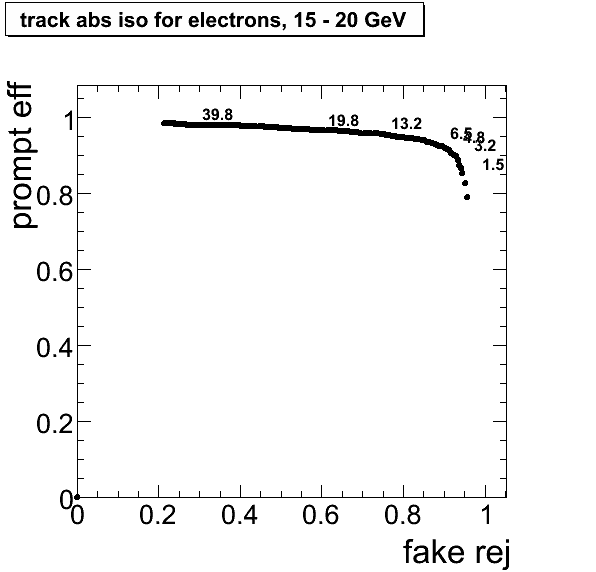
\includegraphics[width = 0.4\textwidth]{pictures/bkgdRej_sigEff/onlyTrack_elec_fake_ptCut2_ptCut3.png}
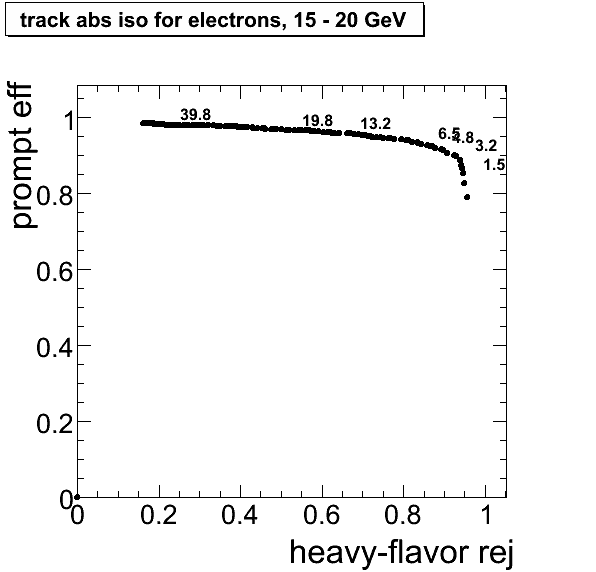
\includegraphics[width = 0.4\textwidth]{pictures/bkgdRej_sigEff/onlyTrack_elec_nonPrompt_ptCut2_ptCut3.png}
\caption{\small{Prompt leptons efficiency with respect to background 
rejection for fake (left) and HF leptons (right) in pT region
from 15 to 20 GeV for electrons. 
Cut values are superimposed to the curve.}\label{fig:rej_el3}}
\end{center}
\end{figure}

\begin{figure}[htbp]
\begin{center}
 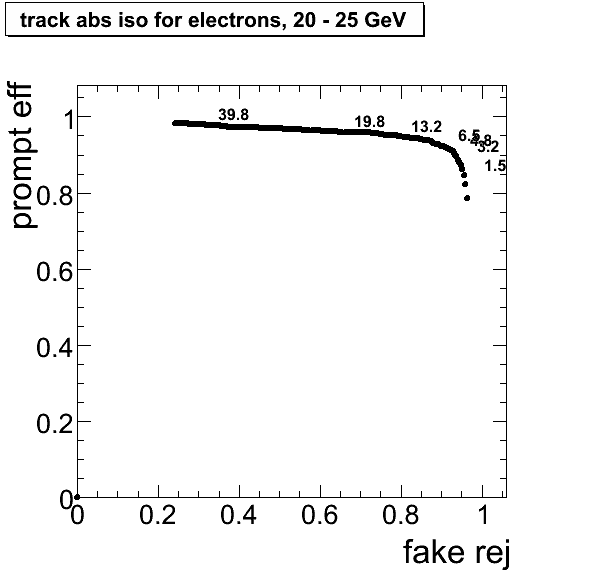
\includegraphics[width = 0.4\textwidth]{pictures/bkgdRej_sigEff/onlyTrack_elec_fake_ptCut3_ptCut4.png}
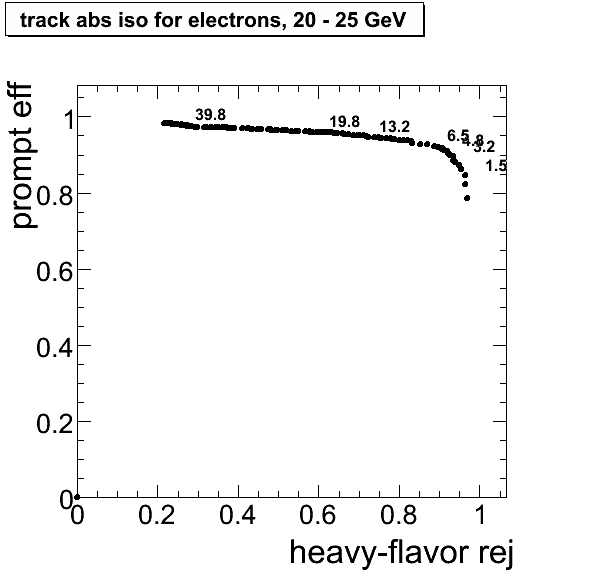
\includegraphics[width = 0.4\textwidth]{pictures/bkgdRej_sigEff/onlyTrack_elec_nonPrompt_ptCut3_ptCut4.png}
\caption{\small{Prompt leptons efficiency with respect to background 
rejection for fake (left) and HF leptons (right) in pT region
from 20 to 25 GeV for electrons. 
Cut values are superimposed to the curve.}\label{fig:rej_el4}}
\end{center}
\end{figure}

\begin{figure}[htbp]
\begin{center}
 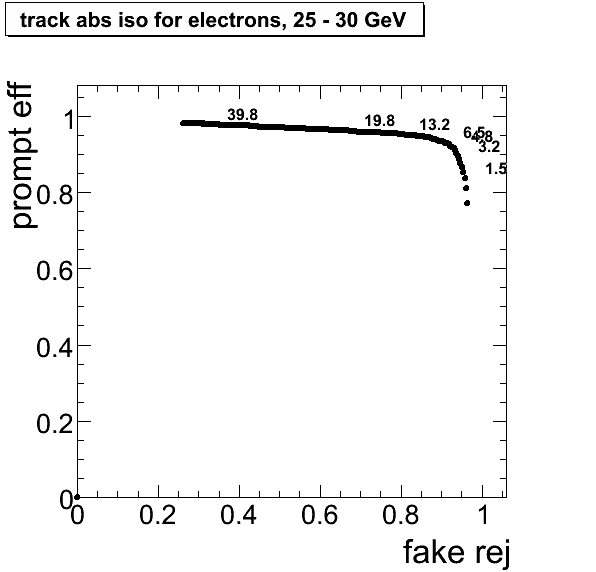
\includegraphics[width = 0.4\textwidth]{pictures/bkgdRej_sigEff/onlyTrack_elec_fake_ptCut4_ptCut5.png}
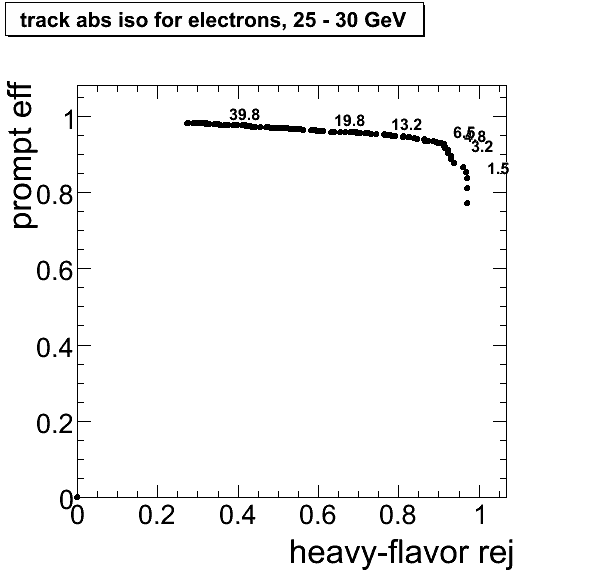
\includegraphics[width = 0.4\textwidth]{pictures/bkgdRej_sigEff/onlyTrack_elec_nonPrompt_ptCut4_ptCut5.png}
\caption{\small{Prompt leptons efficiency with respect to background 
rejection for fake (left) and HF leptons (right) in pT region
from 25 to 30 GeV for electrons. 
Cut values are superimposed to the curve.}\label{fig:rej_el5}}
\end{center}
\end{figure}


\begin{figure}[htbp]
\begin{center}
 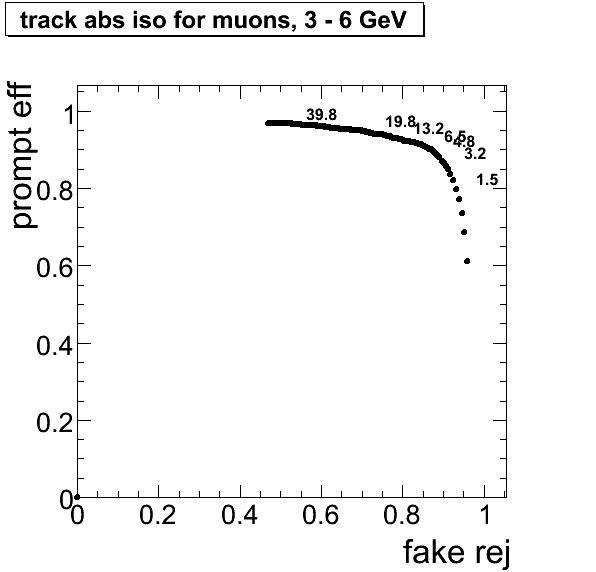
\includegraphics[width = 0.4\textwidth]{pictures/bkgdRej_sigEff/onlyTrack_muon_fake_ptCut0_ptCut1.png}
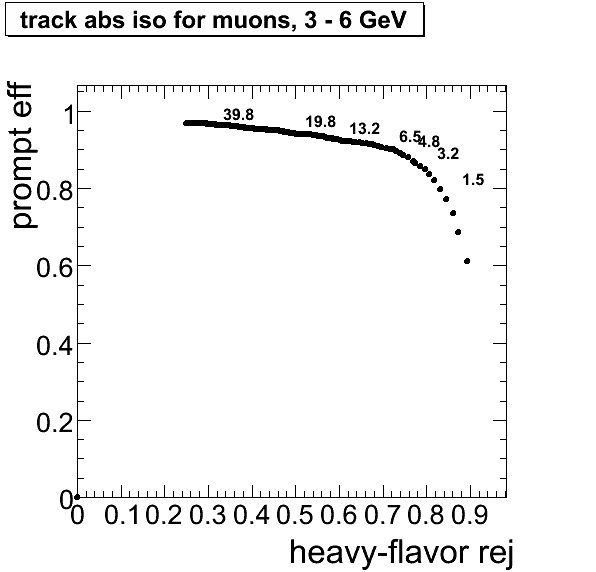
\includegraphics[width = 0.4\textwidth]{pictures/bkgdRej_sigEff/onlyTrack_muon_nonPrompt_ptCut0_ptCut1.png}
\caption{\small{Prompt leptons efficiency with respect to background 
rejection for fake (left) and HF leptons (right) in pT region
from 3 to 6 GeV for muons. 
Cut values are superimposed to the curve.}\label{fig:rej_mu1}}
\end{center}
\end{figure}
\begin{figure}[htbp]
\begin{center}
 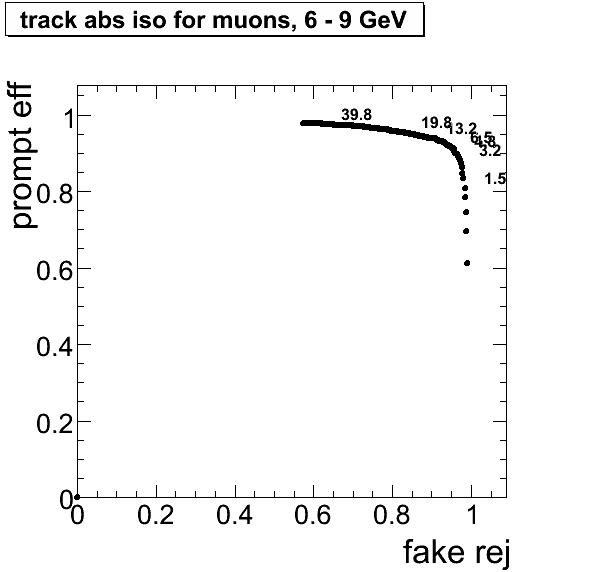
\includegraphics[width = 0.4\textwidth]{pictures/bkgdRej_sigEff/onlyTrack_muon_fake_ptCut1_ptCut2.png}
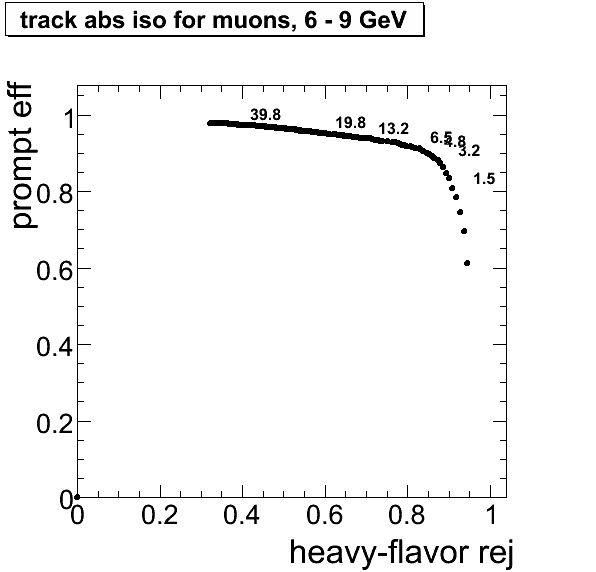
\includegraphics[width = 0.4\textwidth]{pictures/bkgdRej_sigEff/onlyTrack_muon_nonPrompt_ptCut1_ptCut2.png}
\caption{\small{Prompt leptons efficiency with respect to background 
rejection for fake (left) and HF leptons (right) in pT region
from 6 to 9 GeV for muons. 
Cut values are superimposed to the curve.}\label{fig:rej_mu2}}
\end{center}
\end{figure}

\begin{figure}[htbp]
\begin{center}

 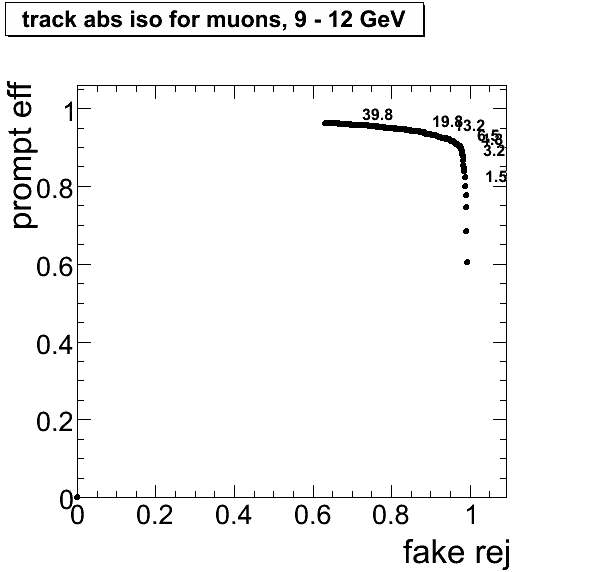
\includegraphics[width = 0.4\textwidth]{pictures/bkgdRej_sigEff/onlyTrack_muon_fake_ptCut2_ptCut3.png}
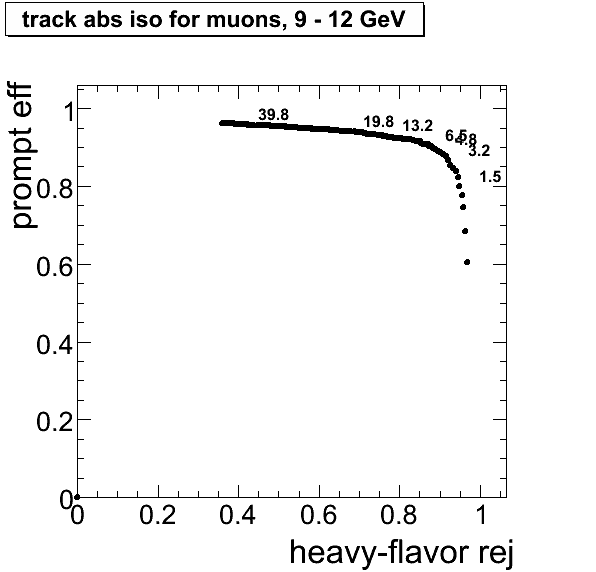
\includegraphics[width = 0.4\textwidth]{pictures/bkgdRej_sigEff/onlyTrack_muon_nonPrompt_ptCut2_ptCut3.png}
\caption{\small{Prompt leptons efficiency with respect to background 
rejection for fake (left) and HF leptons (right) in pT region
from 9 to 12 GeV for muons. 
Cut values are superimposed to the curve.}\label{fig:rej_mu3}}
\end{center}
\end{figure}

\begin{figure}[htbp]
\begin{center}
 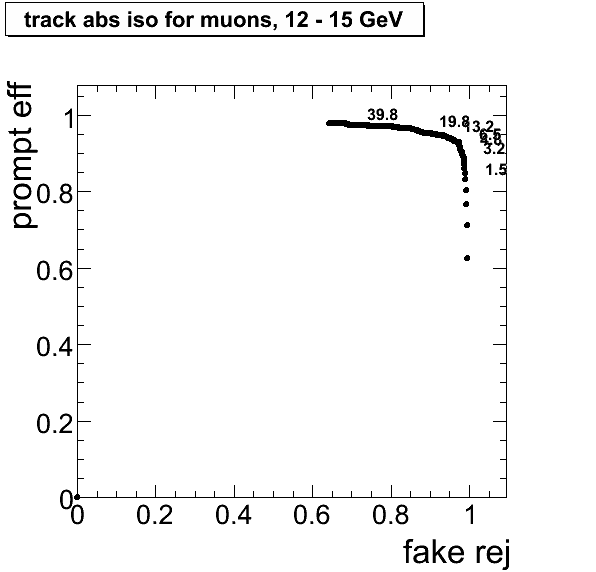
\includegraphics[width = 0.4\textwidth]{pictures/bkgdRej_sigEff/onlyTrack_muon_fake_ptCut3_ptCut4.png}
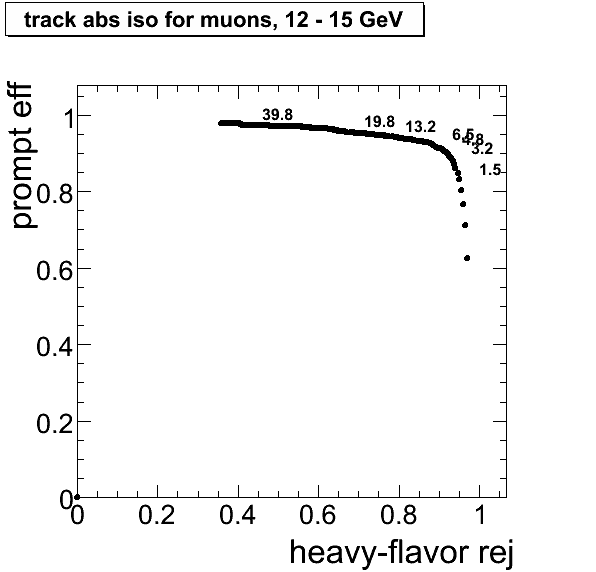
\includegraphics[width = 0.4\textwidth]{pictures/bkgdRej_sigEff/onlyTrack_muon_nonPrompt_ptCut3_ptCut4.png}
\caption{\small{Prompt leptons efficiency with respect to background 
rejection for fake (left) and HF leptons (right) in pT region
from 12 to 15 GeV for muons. 
Cut values are superimposed to the curve.}\label{fig:rej_mu4}}
\end{center}
\end{figure}

\begin{figure}[htbp]
\begin{center}
 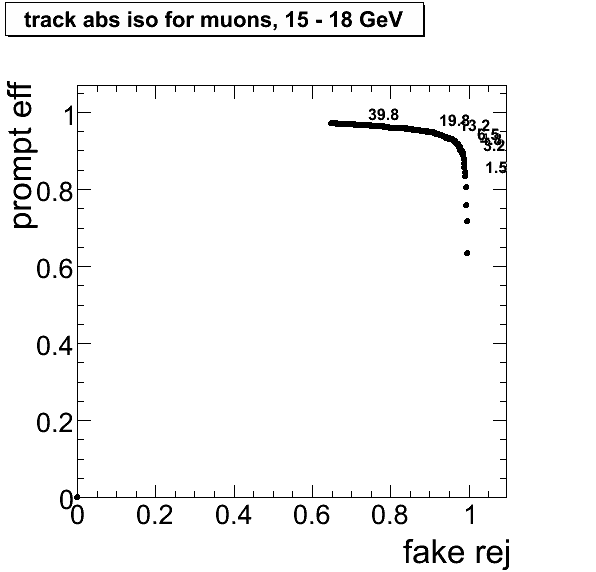
\includegraphics[width = 0.4\textwidth]{pictures/bkgdRej_sigEff/onlyTrack_muon_fake_ptCut4_ptCut5.png}
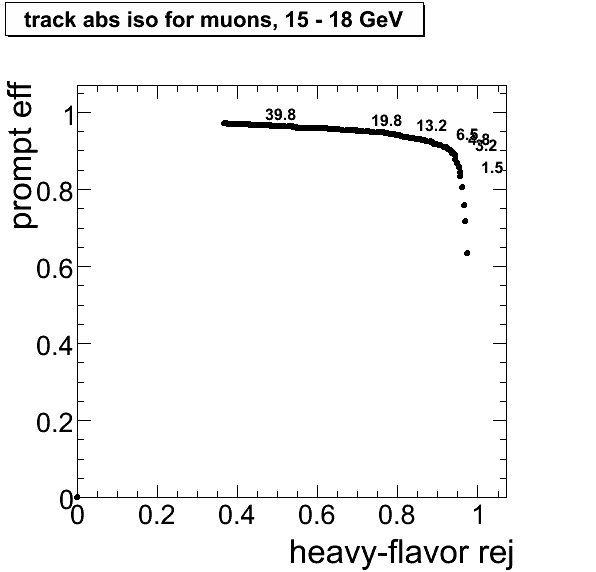
\includegraphics[width = 0.4\textwidth]{pictures/bkgdRej_sigEff/onlyTrack_muon_nonPrompt_ptCut4_ptCut5.png}
\caption{\small{Prompt leptons efficiency with respect to background 
rejection for fake (left) and HF leptons (right) in pT region
from 15 to 18 GeV for muons. 
Cut values are superimposed to the curve.}\label{fig:rej_mu5}}
\end{center}
\end{figure}
\begin{figure}[htbp]
\begin{center}
 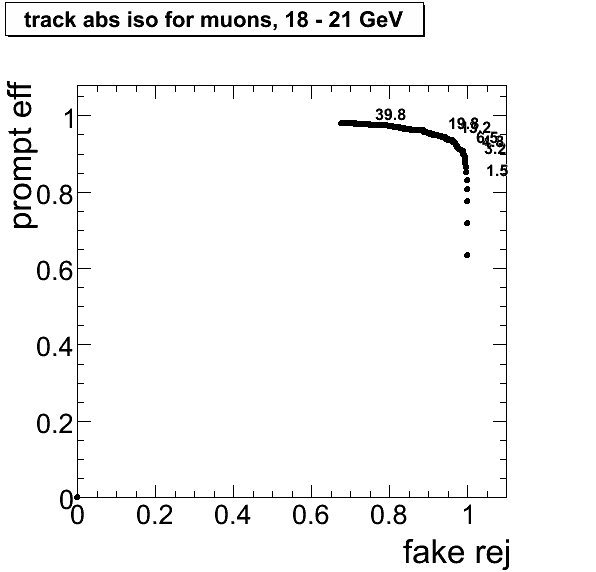
\includegraphics[width = 0.4\textwidth]{pictures/bkgdRej_sigEff/onlyTrack_muon_fake_ptCut5_ptCut6.png}
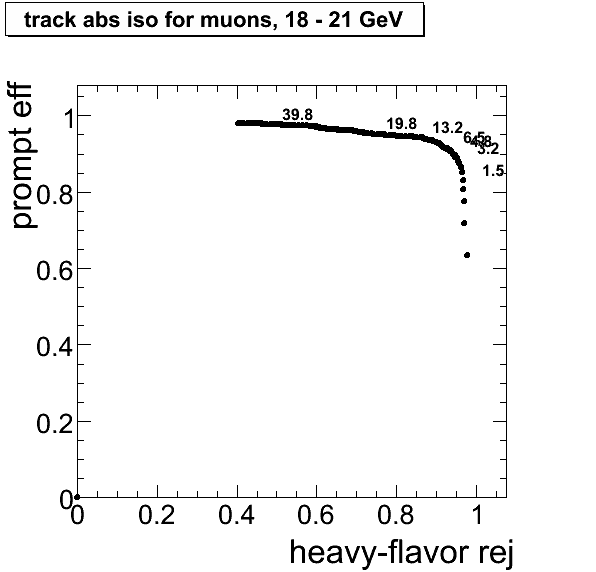
\includegraphics[width = 0.4\textwidth]{pictures/bkgdRej_sigEff/onlyTrack_muon_nonPrompt_ptCut5_ptCut6.png}
\caption{\small{Prompt leptons efficiency with respect to background 
rejection for fake (left) and HF leptons (right) in pT region
from 18 to 21 GeV for muons. 
Cut values are superimposed to the curve.}\label{fig:rej_mu6}}
\end{center}
\end{figure}

\begin{figure}[htbp]
\begin{center}

 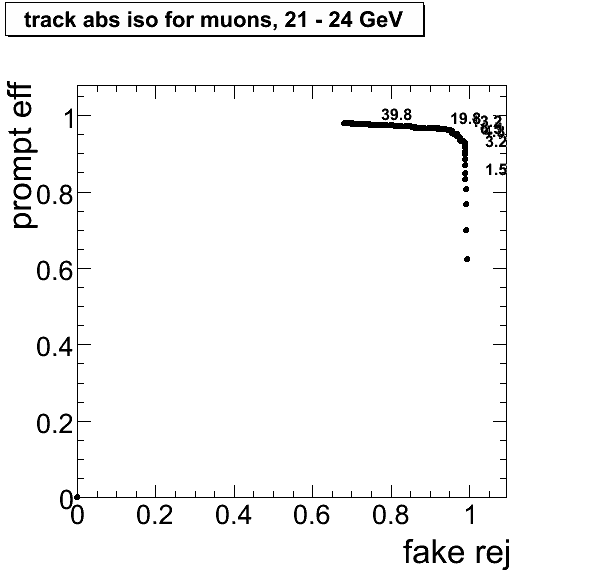
\includegraphics[width = 0.4\textwidth]{pictures/bkgdRej_sigEff/onlyTrack_muon_fake_ptCut6_ptCut7.png}
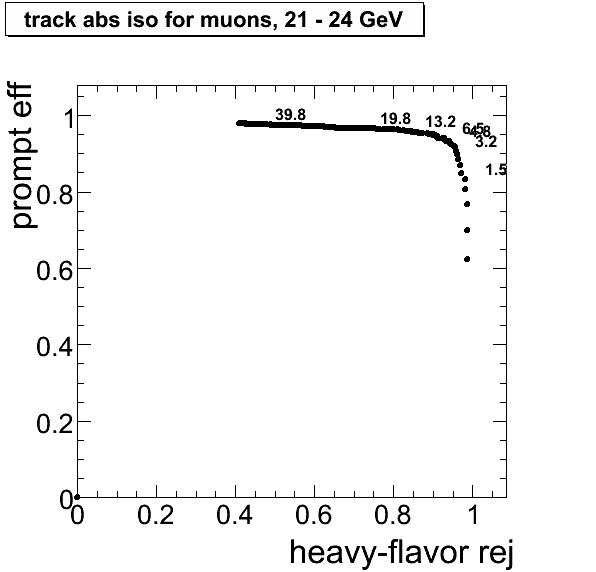
\includegraphics[width = 0.4\textwidth]{pictures/bkgdRej_sigEff/onlyTrack_muon_nonPrompt_ptCut6_ptCut7.png}
\caption{\small{Prompt leptons efficiency with respect to background 
rejection for fake (left) and HF leptons (right) in pT region
from 21 to 24 GeV for muons. 
Cut values are superimposed to the curve.}\label{fig:rej_mu7}}
\end{center}
\end{figure}

\begin{figure}[htbp]
\begin{center}
 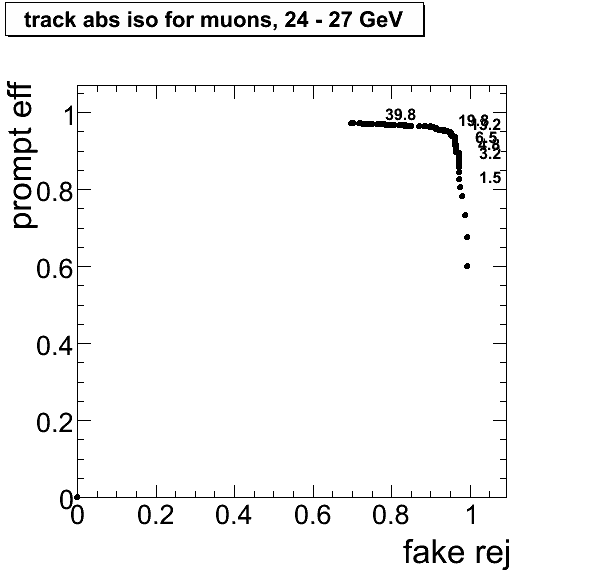
\includegraphics[width = 0.4\textwidth]{pictures/bkgdRej_sigEff/onlyTrack_muon_fake_ptCut7_ptCut8.png}
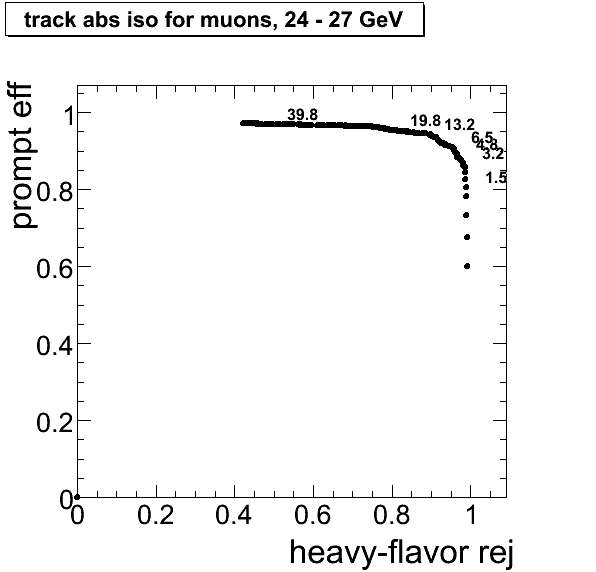
\includegraphics[width = 0.4\textwidth]{pictures/bkgdRej_sigEff/onlyTrack_muon_nonPrompt_ptCut7_ptCut8.png}
\caption{\small{Prompt leptons efficiency with respect to background 
rejection for fake (left) and HF leptons (right) in pT region
from 24 to 27 GeV for muons. 
Cut values are superimposed to the curve.}\label{fig:rej_mu8}}
\end{center}
\end{figure}

\begin{figure}[htbp]
\begin{center}
 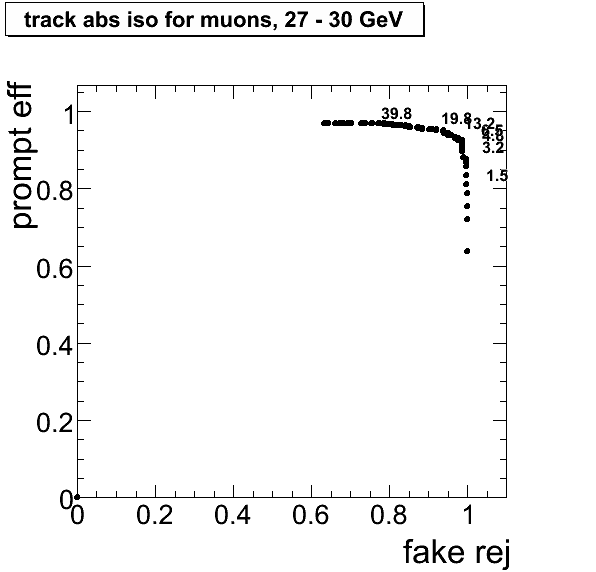
\includegraphics[width = 0.4\textwidth]{pictures/bkgdRej_sigEff/onlyTrack_muon_fake_ptCut8_ptCut9.png}
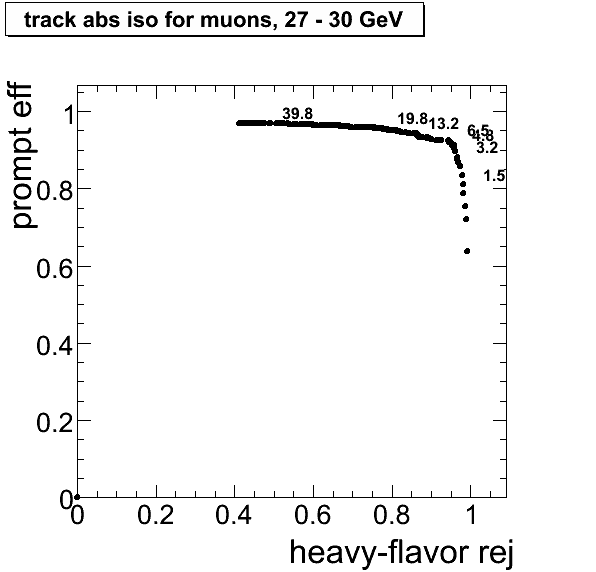
\includegraphics[width = 0.4\textwidth]{pictures/bkgdRej_sigEff/onlyTrack_muon_nonPrompt_ptCut8_ptCut9.png}
\caption{\small{Prompt leptons efficiency with respect to background 
rejection for fake (left) and HF leptons (right) in pT region
from 27 to 30 GeV for muons. 
Cut values are superimposed to the curve.}\label{fig:rej_mu9}}
\end{center}
\end{figure}

\clearpage

\section{Efficiency and rejection plots for ECAL isolation}
\label{sec:ecalplots}
In this appendix the efficiency versus rejection plots are shown for ECAL isolation.
 Efficiency is defined as the number of leptons which pass the 
tracker and ECAL isolation divide by the number of reconstructed leptons

\begin{figure}[htbp]
\begin{center}
 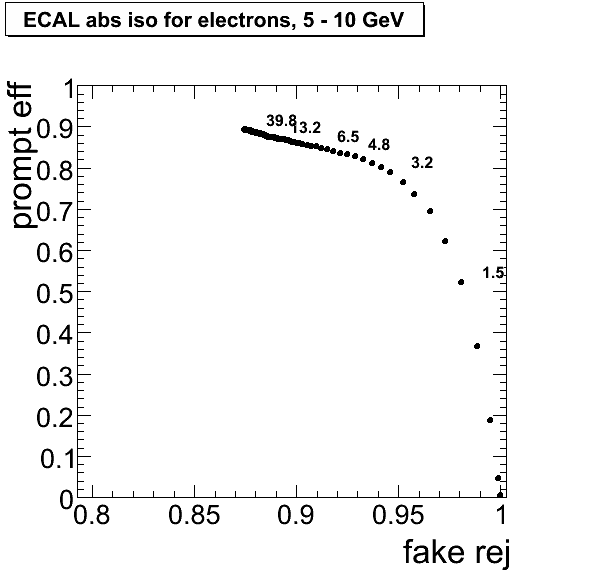
\includegraphics[width = 0.4\textwidth]{pictures/trackCut/bkgdRej_sigEff/elec_fake_ptCut0_ptCut1.png}
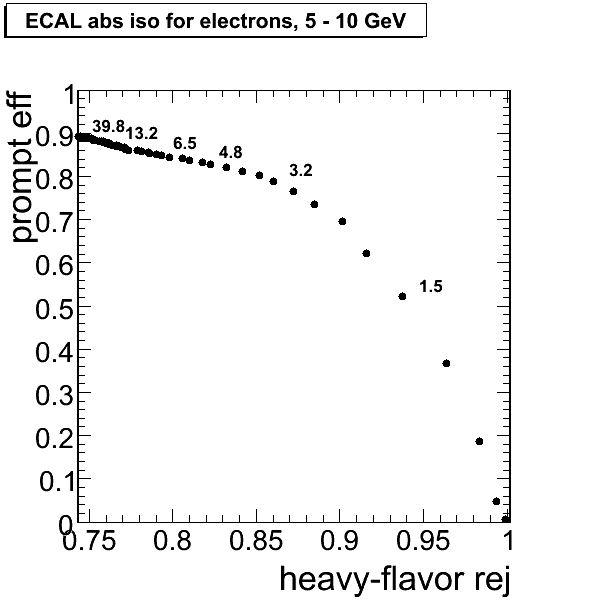
\includegraphics[width = 0.4\textwidth]{pictures/trackCut/bkgdRej_sigEff/elec_nonPrompt_ptCut0_ptCut1.png}
\caption{\small{Prompt leptons efficiency with respect to background 
rejection for fake (left) and HF leptons (right) in pT region
from 5 to 10 GeV for electrons. 
Cut values are superimposed to the curve.}\label{fig:ecalrej_el1}}
\end{center}
\end{figure}
\begin{figure}[htbp]
\begin{center}
 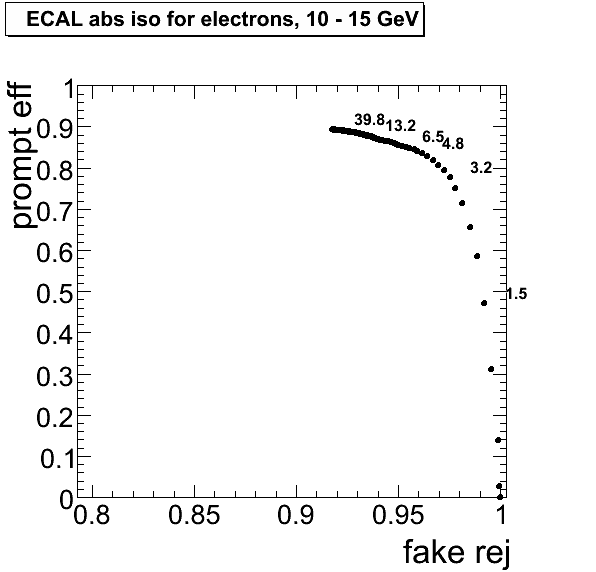
\includegraphics[width = 0.4\textwidth]{pictures/trackCut/bkgdRej_sigEff/elec_fake_ptCut1_ptCut2.png}
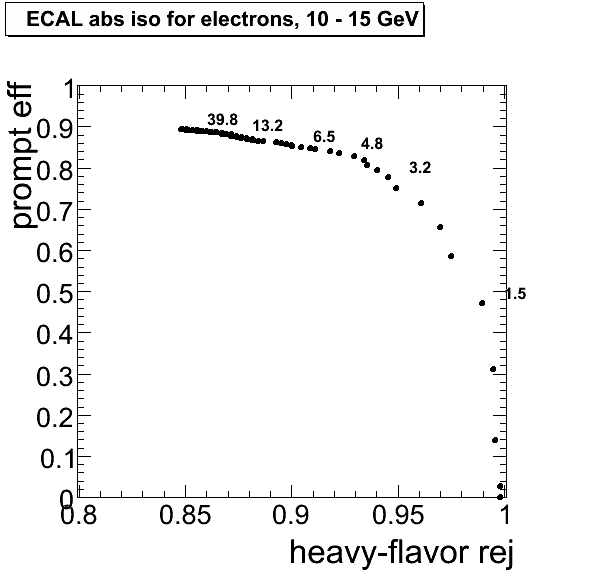
\includegraphics[width = 0.4\textwidth]{pictures/trackCut/bkgdRej_sigEff/elec_nonPrompt_ptCut1_ptCut2.png}
\caption{\small{Prompt leptons efficiency with respect to background 
rejection for fake (left) and HF leptons (right) in pT region
from 10 to 15 GeV for electrons. 
Cut values are superimposed to the curve.}\label{fig:ecalrej_el2}}
\end{center}
\end{figure}

\begin{figure}[htbp]
\begin{center}

 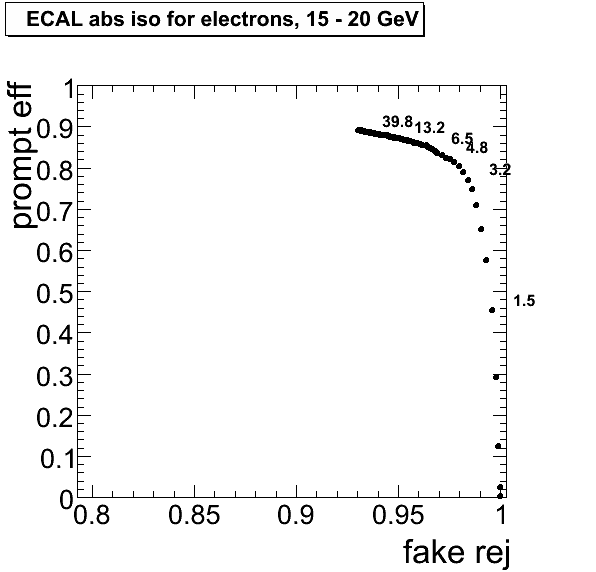
\includegraphics[width = 0.4\textwidth]{pictures/trackCut/bkgdRej_sigEff/elec_fake_ptCut2_ptCut3.png}
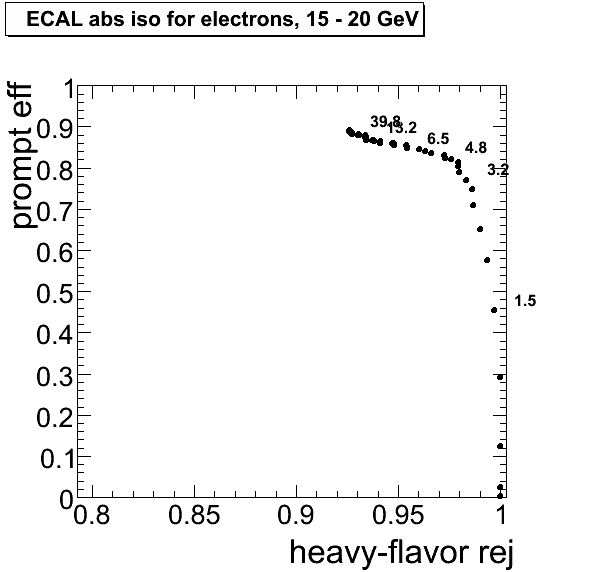
\includegraphics[width = 0.4\textwidth]{pictures/trackCut/bkgdRej_sigEff/elec_nonPrompt_ptCut2_ptCut3.png}
\caption{\small{Prompt leptons efficiency with respect to background 
rejection for fake (left) and HF leptons (right) in pT region
from 15 to 20 GeV for electrons. 
Cut values are superimposed to the curve.}\label{fig:ecalrej_el3}}
\end{center}
\end{figure}

\begin{figure}[htbp]
\begin{center}
 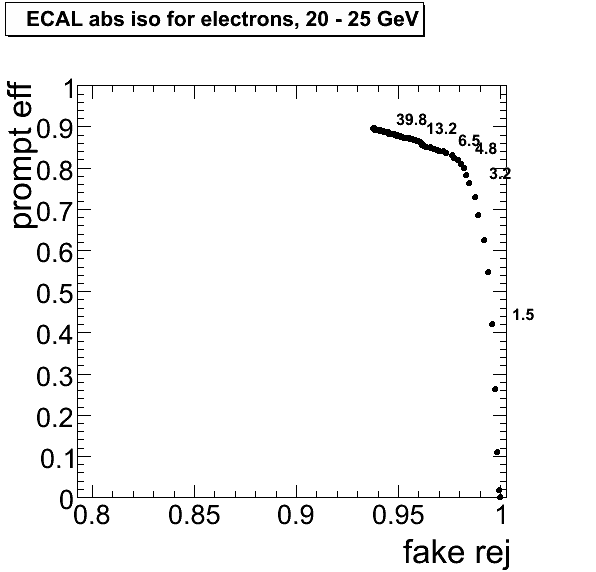
\includegraphics[width = 0.4\textwidth]{pictures/trackCut/bkgdRej_sigEff/elec_fake_ptCut3_ptCut4.png}
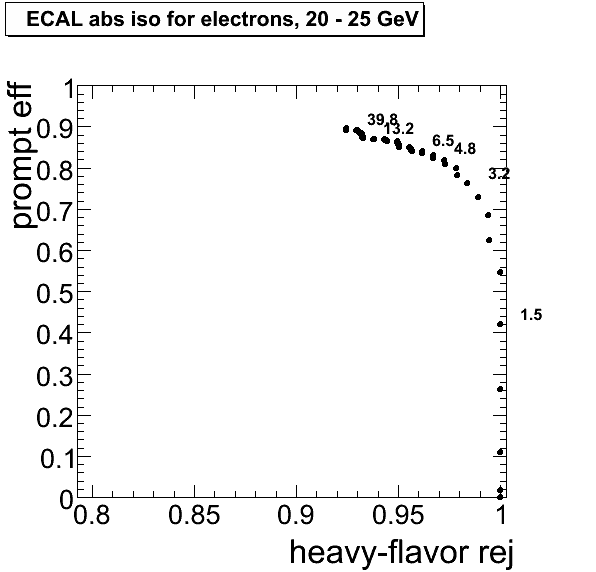
\includegraphics[width = 0.4\textwidth]{pictures/trackCut/bkgdRej_sigEff/elec_nonPrompt_ptCut3_ptCut4.png}
\caption{\small{Prompt leptons efficiency with respect to background 
rejection for fake (left) and HF leptons (right) in pT region
from 20 to 25 GeV for electrons. 
Cut values are superimposed to the curve.}\label{fig:ecalrej_el4}}
\end{center}
\end{figure}

\begin{figure}[htbp]
\begin{center}
 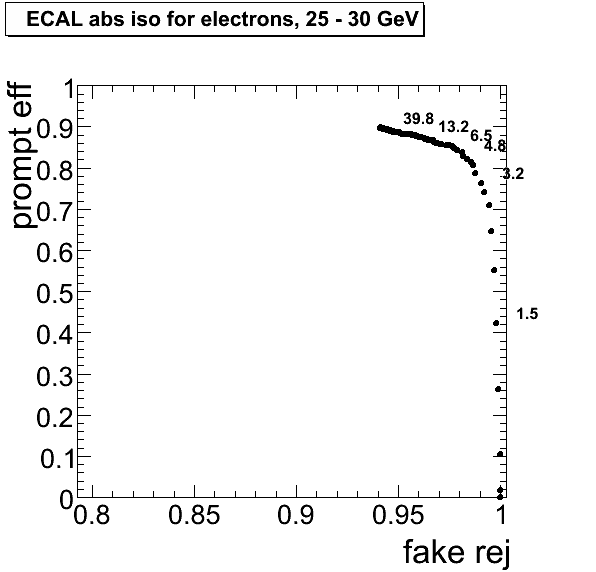
\includegraphics[width = 0.4\textwidth]{pictures/trackCut/bkgdRej_sigEff/elec_fake_ptCut4_ptCut5.png}
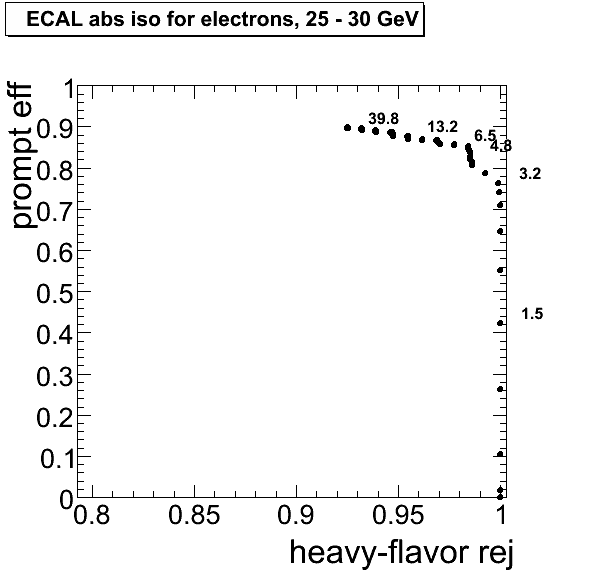
\includegraphics[width = 0.4\textwidth]{pictures/trackCut/bkgdRej_sigEff/elec_nonPrompt_ptCut4_ptCut5.png}
\caption{\small{Prompt leptons efficiency with respect to background 
rejection for fake (left) and HF leptons (right) in pT region
from 25 to 30 GeV for electrons. 
Cut values are superimposed to the curve.}\label{fig:ecalrej_el5}}
\end{center}
\end{figure}


\begin{figure}[htbp]
\begin{center}
 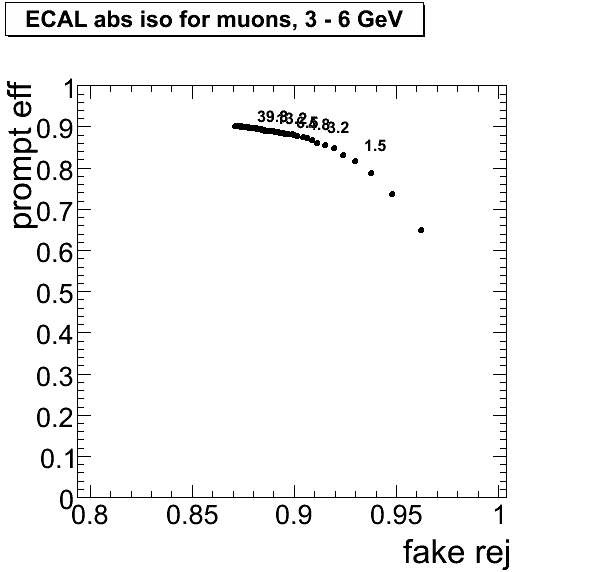
\includegraphics[width = 0.4\textwidth]{pictures/trackCut/bkgdRej_sigEff/muon_fake_ptCut0_ptCut1.png}
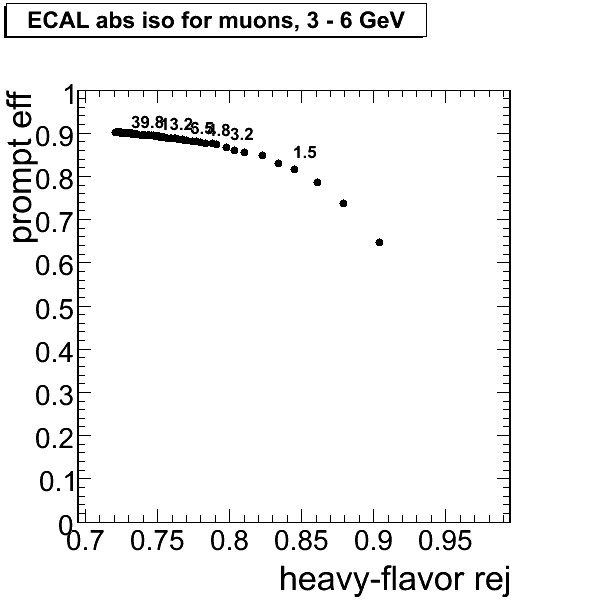
\includegraphics[width = 0.4\textwidth]{pictures/trackCut/bkgdRej_sigEff/muon_nonPrompt_ptCut0_ptCut1.png}
\caption{\small{Prompt leptons efficiency with respect to background 
rejection for fake (left) and HF leptons (right) in pT region
from 3 to 6 GeV for muons. 
Cut values are superimposed to the curve.}\label{fig:ecalrej_mu1}}
\end{center}
\end{figure}
\begin{figure}[htbp]
\begin{center}
 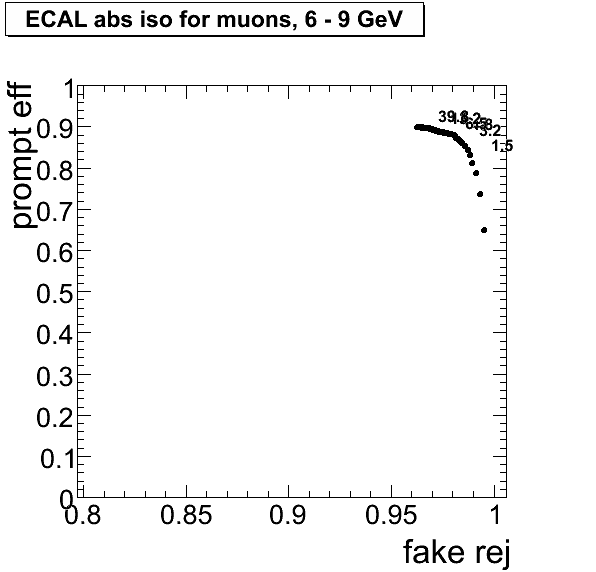
\includegraphics[width = 0.4\textwidth]{pictures/trackCut/bkgdRej_sigEff/muon_fake_ptCut1_ptCut2.png}
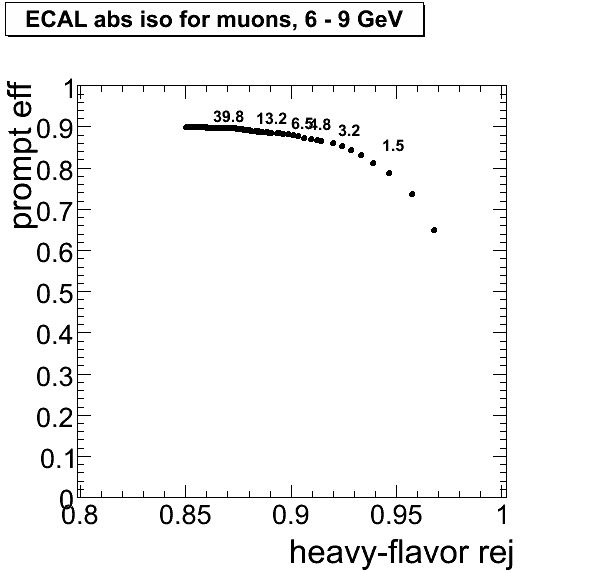
\includegraphics[width = 0.4\textwidth]{pictures/trackCut/bkgdRej_sigEff/muon_nonPrompt_ptCut1_ptCut2.png}
\caption{\small{Prompt leptons efficiency with respect to background 
rejection for fake (left) and HF leptons (right) in pT region
from 6 to 9 GeV for muons. 
Cut values are superimposed to the curve.}\label{fig:ecalrej_mu2}}
\end{center}
\end{figure}

\begin{figure}[htbp]
\begin{center}

 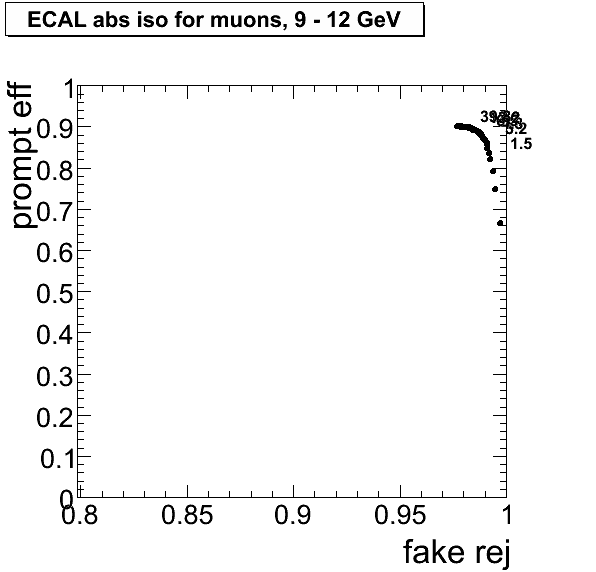
\includegraphics[width = 0.4\textwidth]{pictures/trackCut/bkgdRej_sigEff/muon_fake_ptCut2_ptCut3.png}
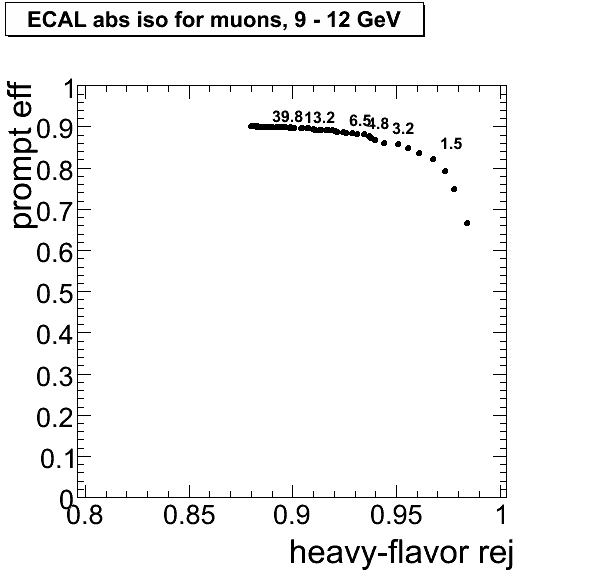
\includegraphics[width = 0.4\textwidth]{pictures/trackCut/bkgdRej_sigEff/muon_nonPrompt_ptCut2_ptCut3.png}
\caption{\small{Prompt leptons efficiency with respect to background 
rejection for fake (left) and HF leptons (right) in pT region
from 9 to 12 GeV for muons. 
Cut values are superimposed to the curve.}\label{fig:ecalrej_mu3}}
\end{center}
\end{figure}

\begin{figure}[htbp]
\begin{center}
 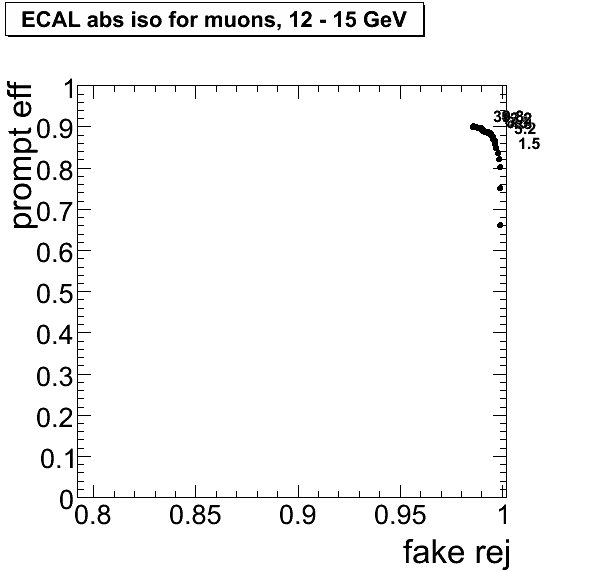
\includegraphics[width = 0.4\textwidth]{pictures/trackCut/bkgdRej_sigEff/muon_fake_ptCut3_ptCut4.png}
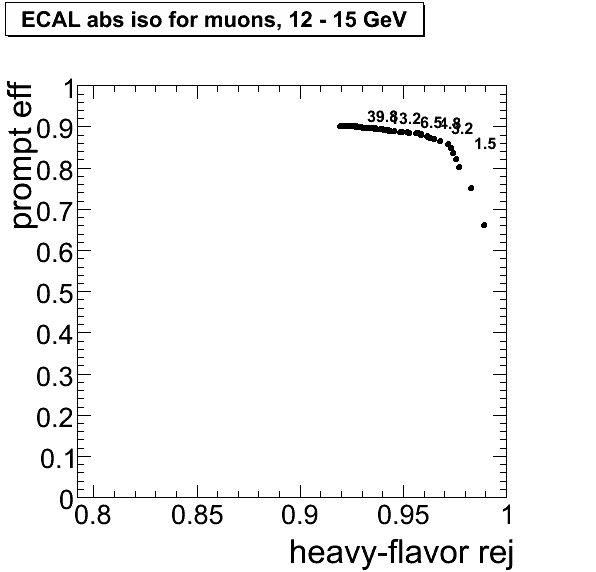
\includegraphics[width = 0.4\textwidth]{pictures/trackCut/bkgdRej_sigEff/muon_nonPrompt_ptCut3_ptCut4.png}
\caption{\small{Prompt leptons efficiency with respect to background 
rejection for fake (left) and HF leptons (right) in pT region
from 12 to 15 GeV for muons. 
Cut values are superimposed to the curve.}\label{fig:ecalrej_mu4}}
\end{center}
\end{figure}

\begin{figure}[htbp]
\begin{center}
 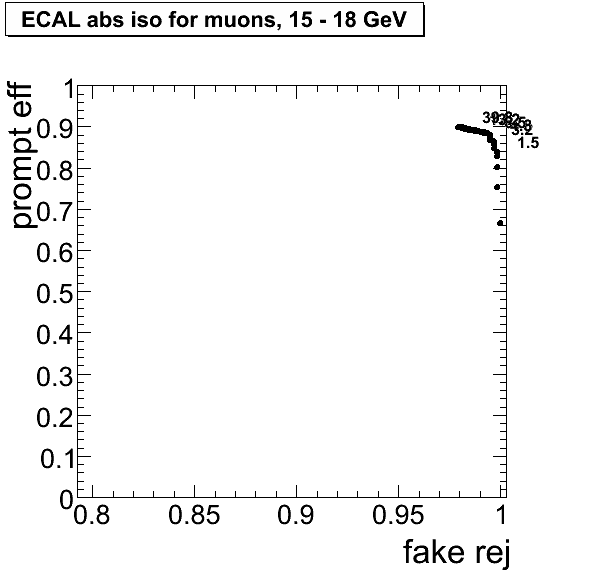
\includegraphics[width = 0.4\textwidth]{pictures/trackCut/bkgdRej_sigEff/muon_fake_ptCut4_ptCut5.png}
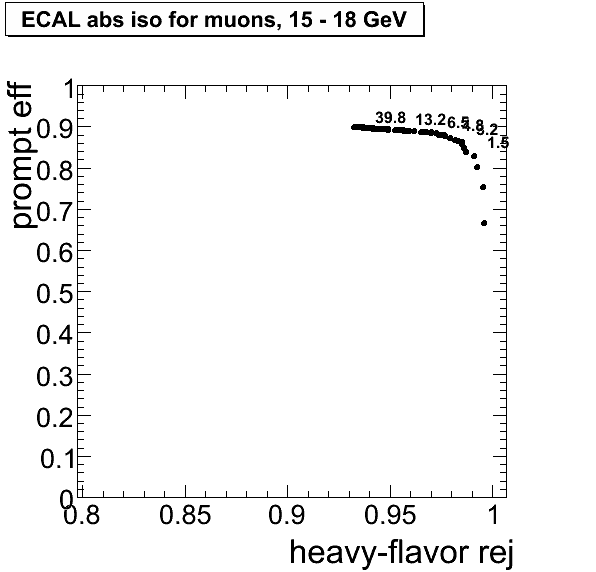
\includegraphics[width = 0.4\textwidth]{pictures/trackCut/bkgdRej_sigEff/muon_nonPrompt_ptCut4_ptCut5.png}
\caption{\small{Prompt leptons efficiency with respect to background 
rejection for fake (left) and HF leptons (right) in pT region
from 15 to 18 GeV for muons. 
Cut values are superimposed to the curve.}\label{fig:ecalrej_mu5}}
\end{center}
\end{figure}

\begin{figure}[htbp]
\begin{center}
 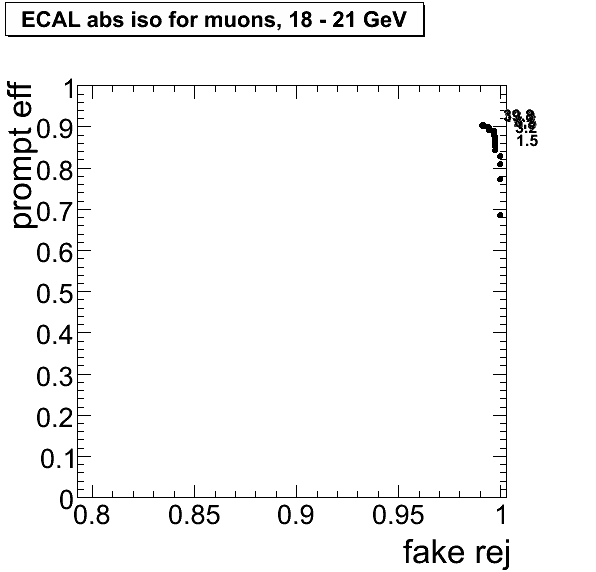
\includegraphics[width = 0.4\textwidth]{pictures/trackCut/bkgdRej_sigEff/muon_fake_ptCut5_ptCut6.png}
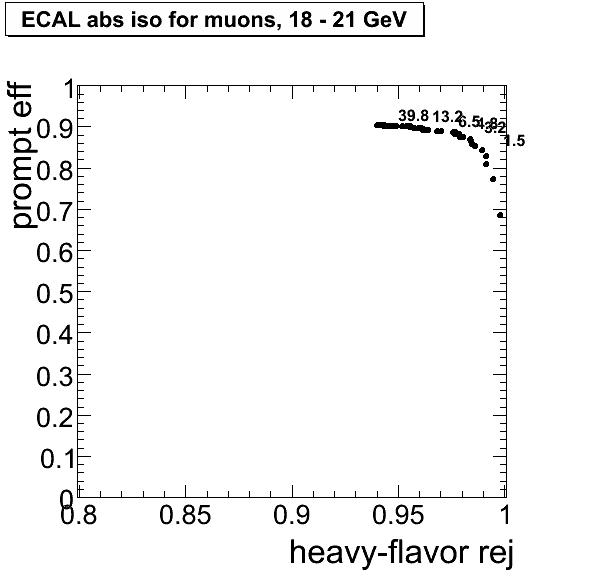
\includegraphics[width = 0.4\textwidth]{pictures/trackCut/bkgdRej_sigEff/muon_nonPrompt_ptCut5_ptCut6.png}
\caption{\small{Prompt leptons efficiency with respect to background 
rejection for fake (left) and HF leptons (right) in pT region
from 18 to 21 GeV for muons. 
Cut values are superimposed to the curve.}\label{fig:ecalrej_mu6}}
\end{center}
\end{figure}

\begin{figure}[htbp]
\begin{center}

 \includegraphics[width = 0.4\textwidth]{pictures/trackCut/bkgdRej_sigEff/muon_fake_ptCut6_ptCut7.png}
\includegraphics[width = 0.4\textwidth]{pictures/trackCut/bkgdRej_sigEff/muon_nonPrompt_ptCut6_ptCut7.png}
\caption{\small{Prompt leptons efficiency with respect to background 
rejection for fake (left) and HF leptons (right) in pT region
from 21 to 24 GeV for muons. 
Cut values are superimposed to the curve.}\label{fig:ecalrej_mu7}}
\end{center}
\end{figure}

\begin{figure}[htbp]
\begin{center}
 \includegraphics[width = 0.4\textwidth]{pictures/trackCut/bkgdRej_sigEff/muon_fake_ptCut7_ptCut8.png}
\includegraphics[width = 0.4\textwidth]{pictures/trackCut/bkgdRej_sigEff/muon_nonPrompt_ptCut7_ptCut8.png}
\caption{\small{Prompt leptons efficiency with respect to background 
rejection for fake (left) and HF leptons (right) in pT region
from 24 to 27 GeV for muons. 
Cut values are superimposed to the curve.}\label{fig:ecalrej_mu8}}
\end{center}
\end{figure}

\begin{figure}[htbp]
\begin{center}
 \includegraphics[width = 0.4\textwidth]{pictures/trackCut/bkgdRej_sigEff/muon_fake_ptCut8_ptCut9.png}
\includegraphics[width = 0.4\textwidth]{pictures/trackCut/bkgdRej_sigEff/muon_nonPrompt_ptCut8_ptCut9.png}
\caption{\small{Prompt leptons efficiency with respect to background 
rejection for fake (left) and HF leptons (right) in pT region
from 27 to 30 GeV for muons. 
Cut values are superimposed to the curve.}\label{fig:ecalrej_mu9}}
\end{center}
\end{figure}
